% \documentclass[11pt,a4paper]{article}
\documentclass[11pt,a4paper]{article}
%%%%%%%%%%%%%%%%%%%%%%%%% Credit %%%%%%%%%%%%%%%%%%%%%%%%

% template ini dibuat oleh martin.manullang@if.itera.ac.id untuk dipergunakan oleh seluruh sivitas akademik itera.

%%%%%%%%%%%%%%%%%%%%%%%%% PACKAGE starts HERE %%%%%%%%%%%%%%%%%%%%%%%%
\usepackage{graphicx}
\usepackage{caption}
\captionsetup[figure]{name=Gambar}
\usepackage{tabulary}   
% \usepackage{amsmath}
\usepackage{fancyhdr}
% \usepackage{amssymb}
% \usepackage{amsthm}
\usepackage{placeins}
% \usepackage{amsfonts}
\usepackage{graphicx}
\usepackage[all]{xy}
\usepackage{tikz}
\usepackage{verbatim}
\usepackage[left=2cm,right=2cm,top=3cm,bottom=2.5cm]{geometry}
\usepackage{hyperref}
\hypersetup{
    colorlinks,
    linkcolor={red!50!black},
    citecolor={blue!50!black},
    urlcolor={blue!80!black}
}
\usepackage{libertine}
\usepackage{libertinust1math}
\usepackage[T1]{fontenc}
\usepackage{inconsolata}

\usepackage{caption}
\usepackage{subcaption}
\usepackage{multirow}
\usepackage{psfrag}
\usepackage[T1]{fontenc}
\usepackage[scaled]{beramono}
% Enable inserting code into the document
\usepackage{listings}
\usepackage{xcolor} 
% custom color & style for listing
\definecolor{codegreen}{rgb}{0,0.6,0}
\definecolor{codegray}{rgb}{0.5,0.5,0.5}
\definecolor{codepurple}{rgb}{0.58,0,0.82}
\definecolor{backcolour}{rgb}{0.95,0.95,0.92}
\lstdefinestyle{mystyle}{
	backgroundcolor=\color{backcolour},   
	commentstyle=\color{green},
	keywordstyle=\color{codegreen},
	numberstyle=\tiny\color{codegray},
	stringstyle=\color{codepurple},
	basicstyle=\ttfamily\footnotesize,
	breakatwhitespace=false,         
	breaklines=true,                 
	captionpos=b,                    
	keepspaces=true,                 
	numbers=left,                    
	numbersep=5pt,                  
	showspaces=false,                
	showstringspaces=false,
	showtabs=false,                  
	tabsize=2
}
\lstset{style=mystyle}
\renewcommand{\lstlistingname}{Kode}
%%%%%%%%%%%%%%%%%%%%%%%%% PACKAGE ends HERE %%%%%%%%%%%%%%%%%%%%%%%%


%%%%%%%%%%%%%%%%%%%%%%%%% Data Diri %%%%%%%%%%%%%%%%%%%%%%%%
\newcommand{\stuid}{120140116}
\newcommand{\student}{\textbf{Muhammad Qomarudin (\stuid{})}}
\newcommand{\course}{\textbf{Sistem Operasi (IF2223)}}
\newcommand{\assignment}{\textbf{01}} % tugas ke...

%%%%%%%%%%%%%%%%%%% using theorem style %%%%%%%%%%%%%%%%%%%%
\newtheorem{thm}{Theorem}
\newtheorem{lem}[thm]{Lemma}
\newtheorem{defn}[thm]{Definition}
\newtheorem{exa}[thm]{Example}
\newtheorem{rem}[thm]{Remark}
\newtheorem{coro}[thm]{Corollary}
\newtheorem{quest}{Question}[section]
%%%%%%%%%%%%%%%%%%%%%%%%%%%%%%%%%%%%%%%%
\usepackage{lipsum}%% a garbage package you don't need except to create examples.
\usepackage{fancyhdr}
\usepackage[ddmmyyyy]{datetime}
\pagestyle{fancy}
\lhead{ \student }
\rhead{ \thepage}
\cfoot{\textbf{Judul Tugas diketik di sini}} % ini untuk judul tugas
\renewcommand{\headrulewidth}{0.4pt}
\renewcommand{\footrulewidth}{0.4pt}

%%%%%%%%%%%%%%  Shortcut for usual set of numbers  %%%%%%%%%%%

\newcommand{\N}{\mathbb{N}}
\newcommand{\Z}{\mathbb{Z}}
\newcommand{\Q}{\mathbb{Q}}
\newcommand{\R}{\mathbb{R}}
\newcommand{\C}{\mathbb{C}}
\setlength\headheight{14pt}

%%%%%%%%%%%%%%%%%%%%%%%%%%%%%%%%%%%%%%%%%%%%%%%%%%%%%%%555

\begin{document}
\thispagestyle{empty}
\begin{center}
	
\includegraphics[scale = 0.15]{Figure/ifitera-header.png}
	\vspace{0.1cm}
\end{center}
\noindent
% change font family for header section only
%{\fontfamily{LinuxLibertineT-OsF}\large\selectfont 
{\large
\rule{17cm}{0.2cm}\\[0.3cm]
Nama: \student \hfill Tugas Ke: \assignment\\[0.1cm]
Mata Kuliah: \course \hfill Tanggal: \today\\
\rule{17cm}{0.05cm}
\vspace{0.1cm}
}


%%%%%%%%%%%%%%%%%%%%%%%%%%%%%%%%%%%%%%%%%%%%% BODY DOCUMENT %%%%%%%%%%%%%%%%%%%%%%%%%%%%%%%%%%%%%%%%%%%%%
\section{Header Pertama}
    Untuk menggunakan header, anda cukup membuat $\backslash${\tt{section}} pada bagian script anda. Penomoran pada header akan otomatis dibuat. Jika anda membutuhkan line break, anda dapat membubuhkan dua garis miring dengan backslash seperti berikut $\backslash\backslash$

\section{Cara Mencantumkan Link}
    Anda dapat memulai belajar menulis di \LaTeX dengan menulis tugas atau laporan yang sesungguhnya. Pada awalnya mungkin terasa sulit. Namun jika anda dengan tekun tetap berlatih, justru menulis di LaTeX akan membuat anda terbiasa dan malah lebih menyenangkan ketimbang menulis di Microsoft Word.\\
    Jika anda ingin mencantumkan link di \LaTeX anda dapat melakukannya dengan perintah $\backslash${\tt{href}}, misalnya pada tautan berikut ini \href{http://aldi_tob_2000.staff.gunadarma.ac.id/Downloads/files/17359/Membuat+dokumen+dengan+latex.pdf}{(Sumber: PDF Tutorial Belajar Latex)}.
    
\subsection{Sub Header atau Sub Chapter}
     Untuk menggunakan subheader, anda cukup membuat $\backslash${\tt{subsection}} atau bahkan  $\backslash${\tt{subsubsection}} untuk sub-sub bab. Lalu bagaimana untuk membuat subheader atau bahkan header namun tanpa penomoran? Cek keterangan di bawah ini.

\subsection*{Sub Header atau Sub Chapter}
    Untuk menggunakan subheader, anda cukup membuat $\backslash${\tt{subsection}} atau bahkan  $\backslash${\tt{subsubsection}} untuk sub-sub bab. Lalu bagaimana untuk membuat subheader atau bahkan header namun tanpa penomoran? Cek keterangan di bawah ini.
\subsection*{Sub Caption}
    Untuk menggunakan subcaption, anda cukup membuat $\backslash${\tt{subcaption}} atau bahkan  $\backslash${\tt{subsubcaption}} untuk sub-sub bab. Lalu bagaimana untuk membuat subcaption atau bahkan caption namun tanpa penomoran? Cek keterangan di bawah ini.
\subsection{Bold, Italic, Plaintext}
\begin{itemize}
    \item Anda dapat membuat cetak tebal dengan perintah $\backslash${\tt{textbf}} seperti \textbf{berikut ini}.
    \item Anda dapat membuat cetak miring dengan perintah $\backslash${\tt{textit}} seperti \textit{berikut ini}. \item Untuk menggaris bawahi, tinggal ketikkan perintah $\backslash${\tt{underline}} seperti \underline{berikut ini}.
    \item Untuk membuat list seperti tulisan ini, gunakan perintah $\backslash${\tt{item}} diantara
\end{itemize}

\subsection{Code Snippets}
    Berikut ini adalah contoh dari penggunaan $\backslash${\tt{begin{lstlisting}}} untuk menulis potongan kode. Dalam kasus ini saya menggunakan bahasa Python. Jika anda menggunakan C atau yang lainnya, tinggal sesuaikan di bagian parameter dari $\backslash${\tt{begin{lstlisting}}}. Anda dapat melihatnya pada code snipptes \ref{labelkode}
    
    \begin{lstlisting}[language=Python, caption=Captionnya tulis di sini class,label={labelkode}]
    class SynthiaDataset(Dataset):

    CLASSES = [
        "void", "road", "sidewalk", "building", "wall", "fence", "pole", "traffic light", 
        "traffic sign", "vegetation", "terrain", "sky", "person", "rider", "car", "truck", 
        "bus", "train", "motorcycle", "bicycle", "road lines", "other", "road works"
    ]
    
    def __init__(self, path="../SYNTHIA-SF", classes=None, augmentation=None, preprocessing=None, valid=False):
        self.rootdir = Path(path)
        self.data_imgs, self.data_gts = self.prepare_data(valid,path)
        self.valid = valid

    
        if classes == None:
            classes = self.CLASSES 
        self.class_values = [self.CLASSES.index(cls.lower()) for cls in classes]
        
        self.augmentation = augmentation
        self.preprocessing = preprocessing
    \end{lstlisting}

\section{Memuat Multi-Gambar}
Berikut ini adalah contoh cara untuk memuat multi-gambar.

\begin{figure}[h]
	\centering
	\begin{subfigure}[b]{0.4\textwidth}
		\centering
		\def\svgwidth{\columnwidth}
		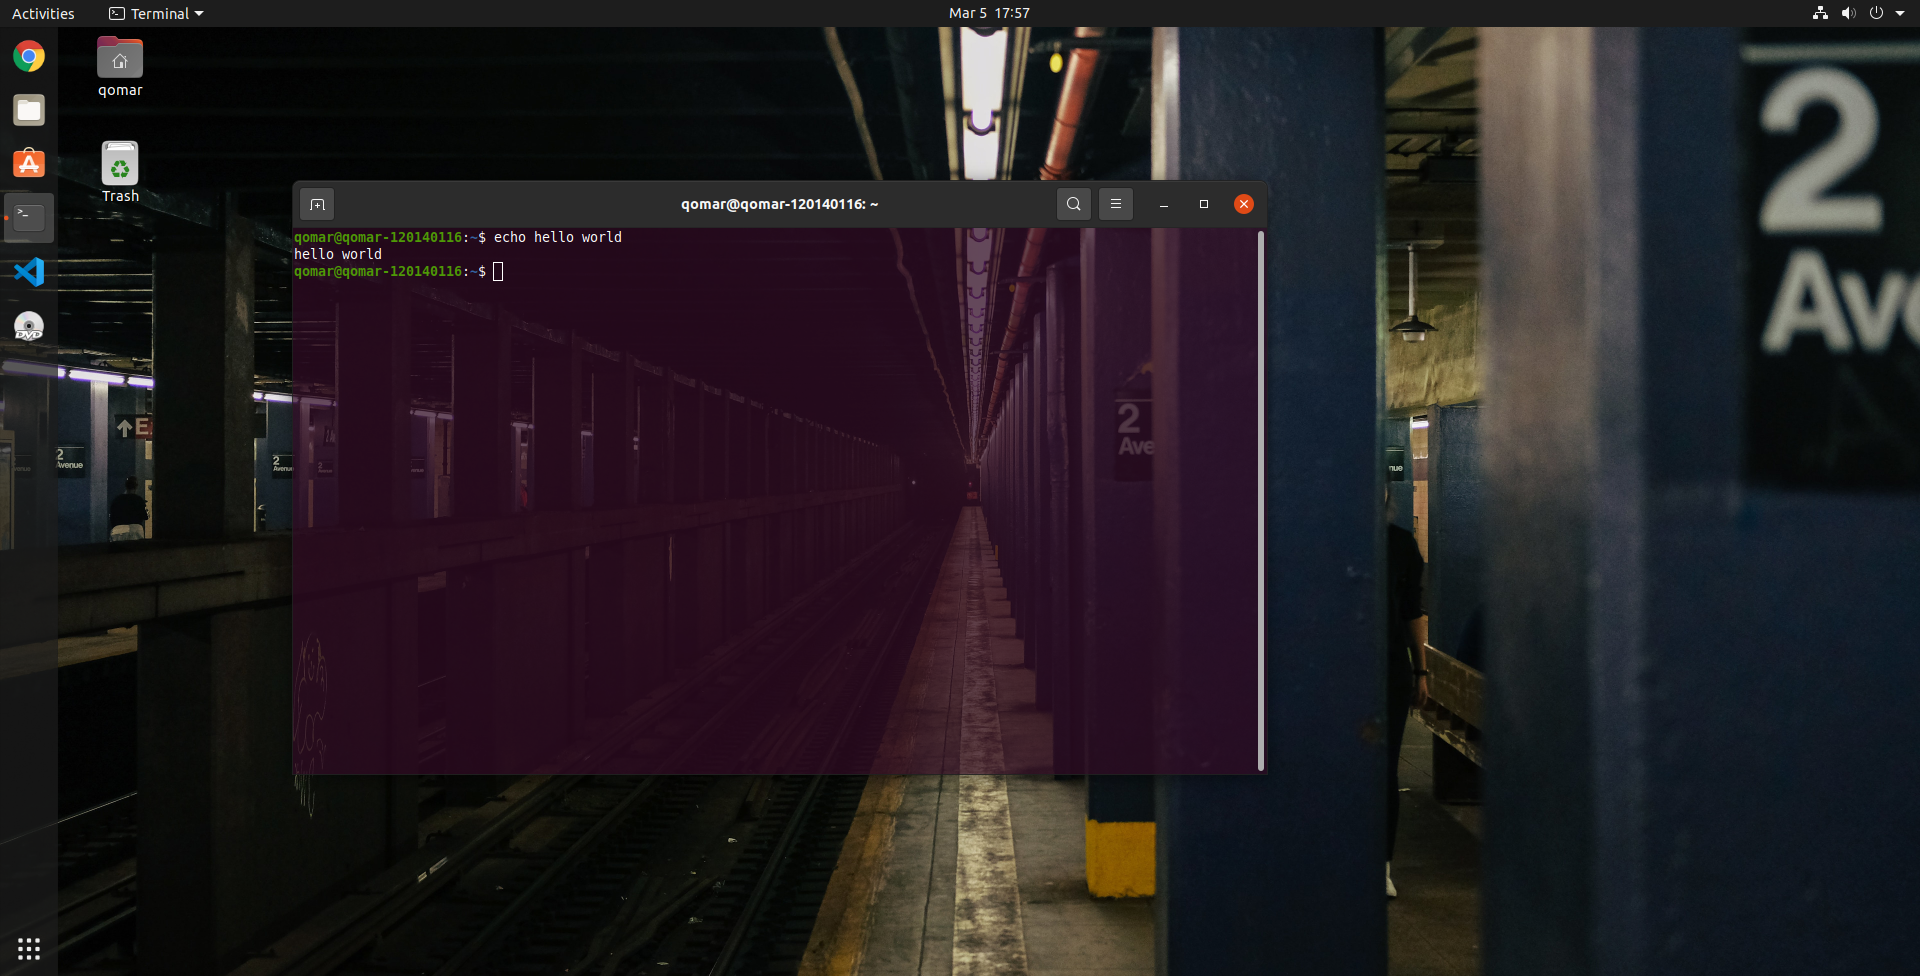
\includegraphics[width=1\textwidth]{figure/tut1_bagian1.png}
		\caption{Augment Result 1}
		\label{fig:aug-1}
	\end{subfigure}
	\qquad %add desired spacing between images, e. g. ~, \quad, \qquad, \hfill etc. 
	%(or a blank line to force the subfigure onto a new line)
	\begin{subfigure}[b]{0.4\textwidth}
		\centering
		\def\svgwidth{\columnwidth}
		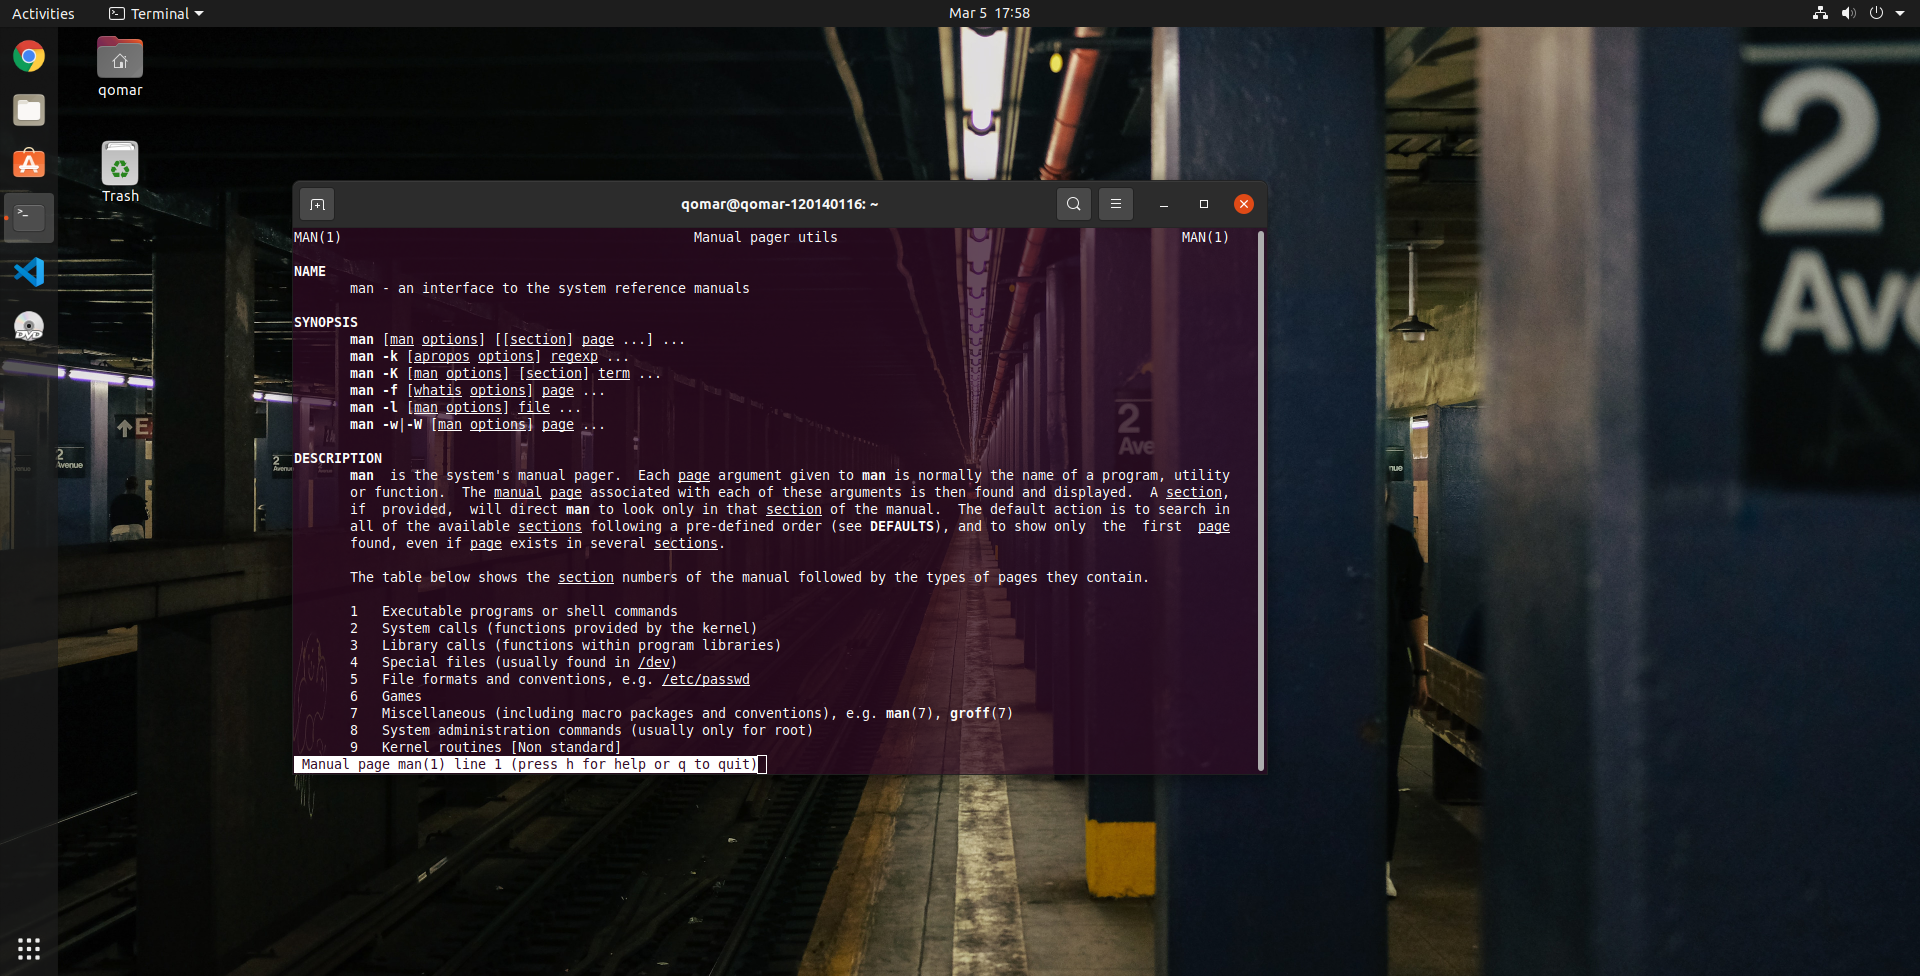
\includegraphics[width=1\textwidth]{figure/tut1_bagian2.png}
		\caption{Augment Result 2}
		\label{fig:aug-2}
	\end{subfigure}
	\caption{Augmentation Samples}\label{fig:aug}
\end{figure}


\newpage
\section{Memuat Multi-Gambar}
Berikut ini adalah contoh cara untuk memuat multi-gambar.
\newpage
\bibliographystyle{IEEEtran}
\bibliography{Referensi}
\end{document}